\documentclass{beamer}
\usetheme{metropolis}
\usepackage{ctex}
\usepackage{caption}
\usepackage{subfigure}
\usepackage{listings}

\title{Item-Based Collaborative Filtering}
\date{\today}
\author{Yang LI}
\institute{School of Software Engineering, Tongji University}

\begin{document}
  \maketitle
  \section{Chinese Text Segmentation}
  \begin{frame}{分词的优化}
    加入原数据的品牌名作为自定义词典, 提供给分词算法.\\
    Precision:
    \begin{figure}
      \centering
      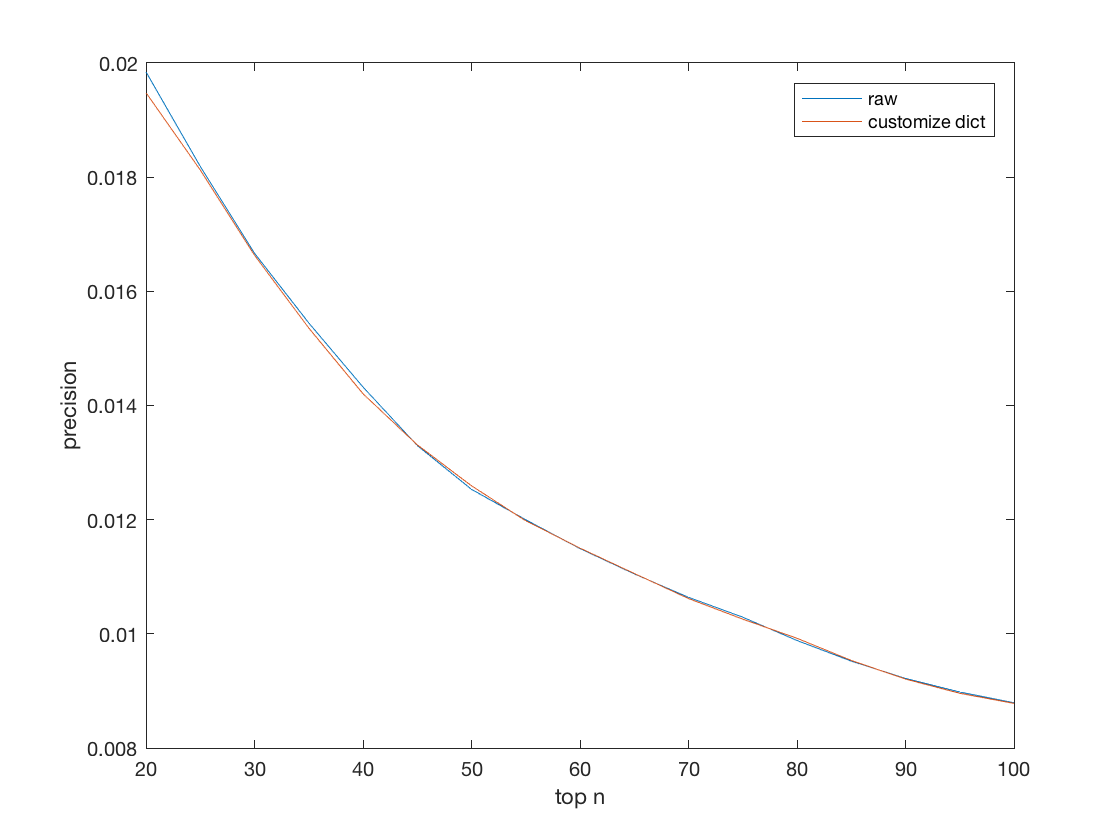
\includegraphics[width=0.9\textwidth]{Nov-16/fig1.png}
    \end{figure}
  \end{frame}
  \begin{frame}{分词的优化}
    Recall:
    \begin{figure}
      \centering
      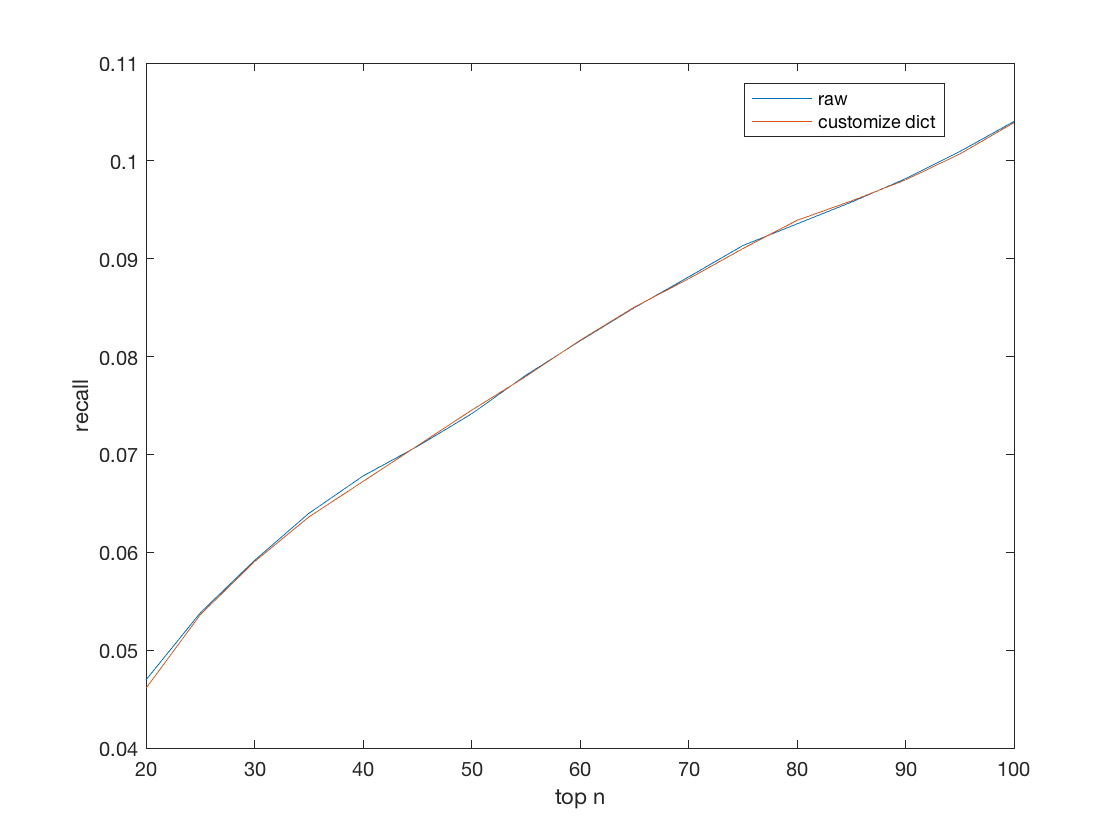
\includegraphics[width=0.9\textwidth]{Nov-16/fig2.png}
    \end{figure}
  \end{frame}

  \section{Item Cosine Similarity}
  \begin{frame}{商品距离的优化}
    使用了高斯距离.\\
    Precision:
    \begin{figure}
      \centering
      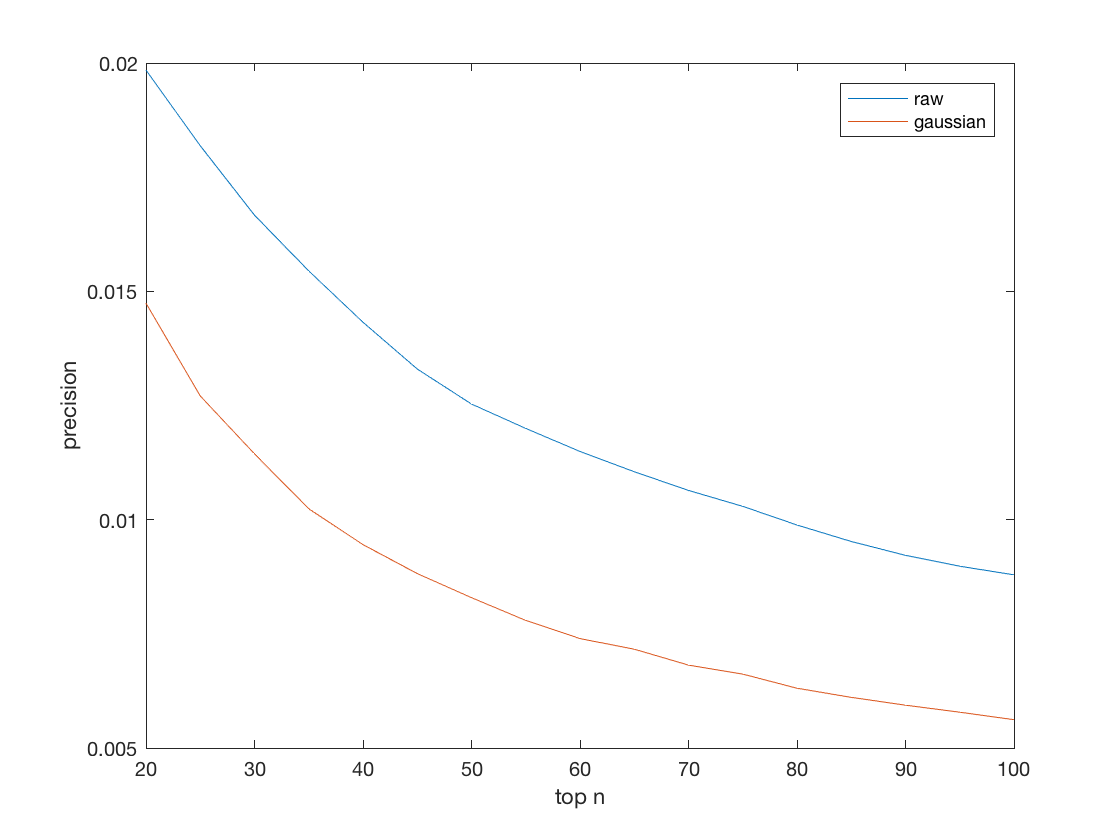
\includegraphics[width=0.9\textwidth]{Nov-16/fig3.png}
    \end{figure}
  \end{frame}
    \begin{frame}{商品距离的优化}
    Recall:
    \begin{figure}
      \centering
      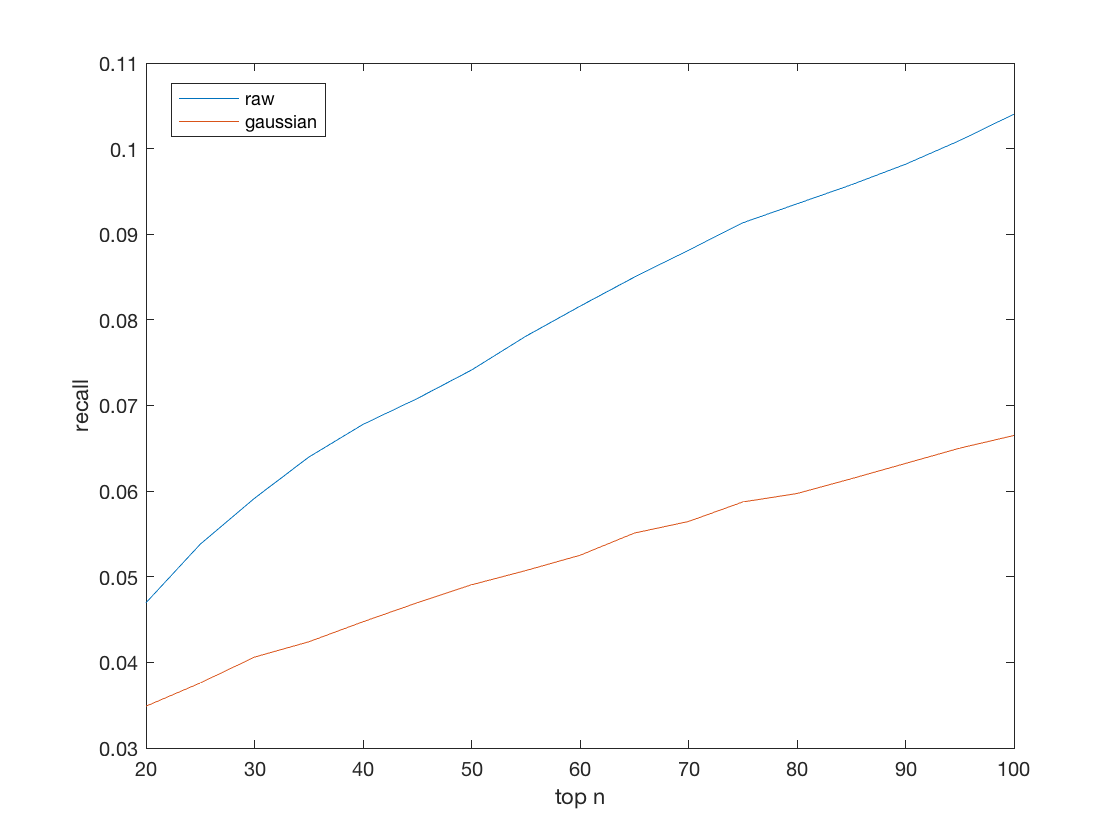
\includegraphics[width=0.9\textwidth]{Nov-16/fig4.png}
    \end{figure}
  \end{frame}
  \begin{frame}
    对多个Gaussian的Sigma进行测试:\\
    prev: $Sigma = 10$
    \begin{figure}
      \centering
      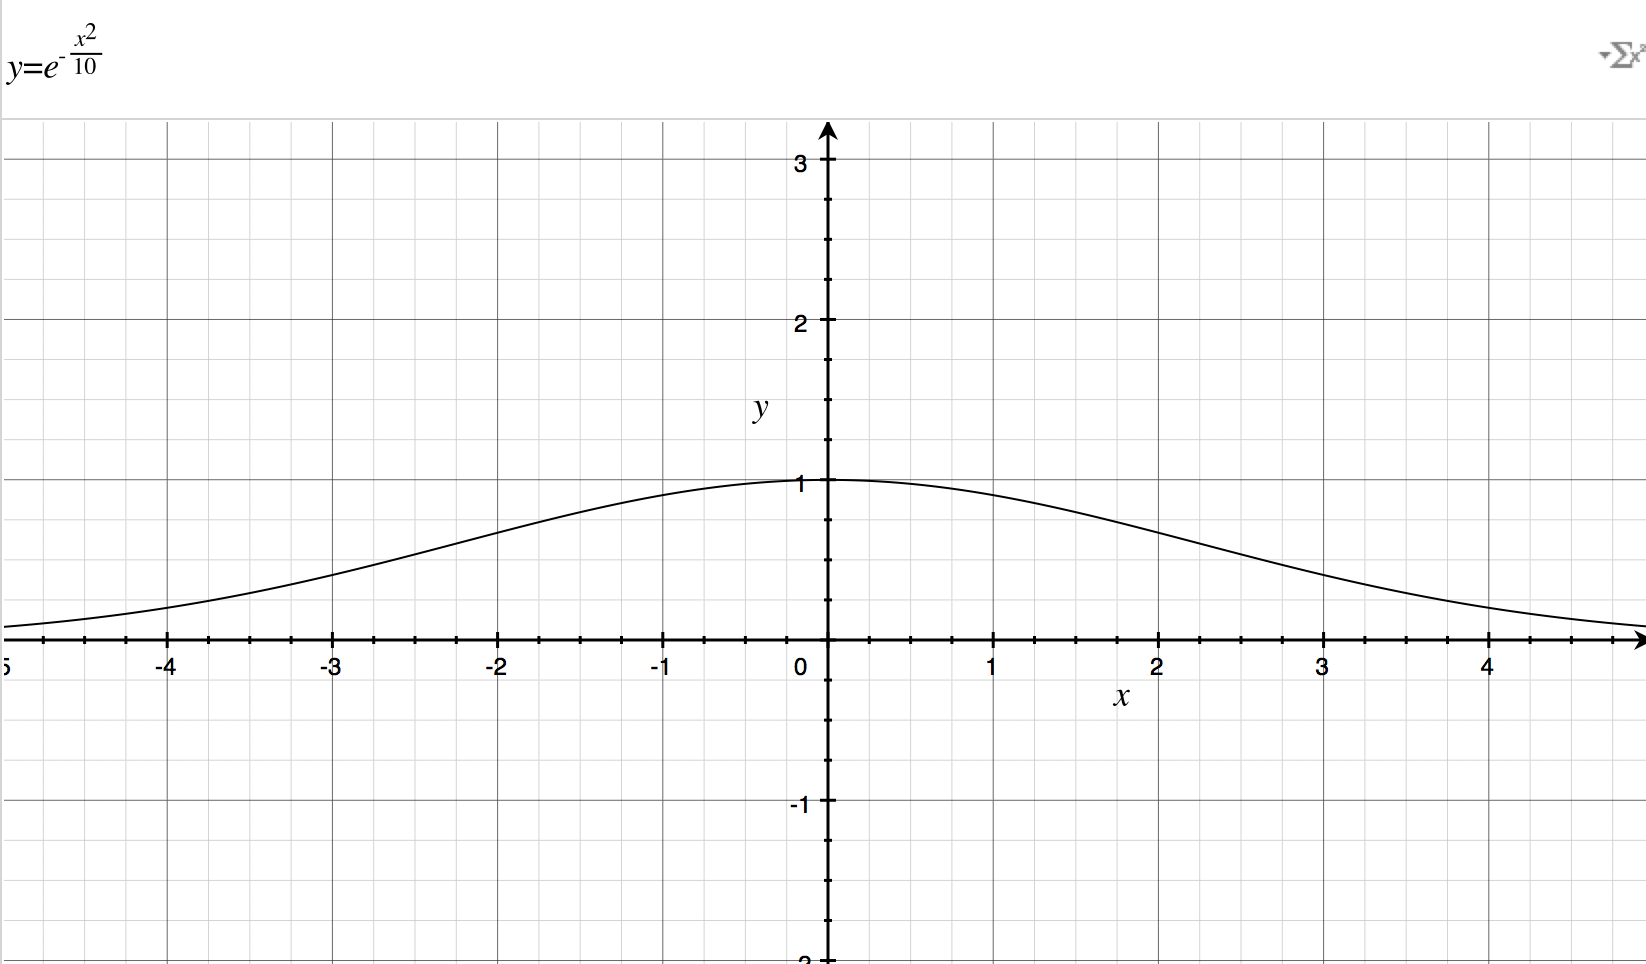
\includegraphics[width=0.9\textwidth]{Nov-16/fig7.png}
    \end{figure}
  \end{frame}
  
  \section{Other Attempts}
  \begin{frame}{分割量词}
    \begin{figure}
      \centering
      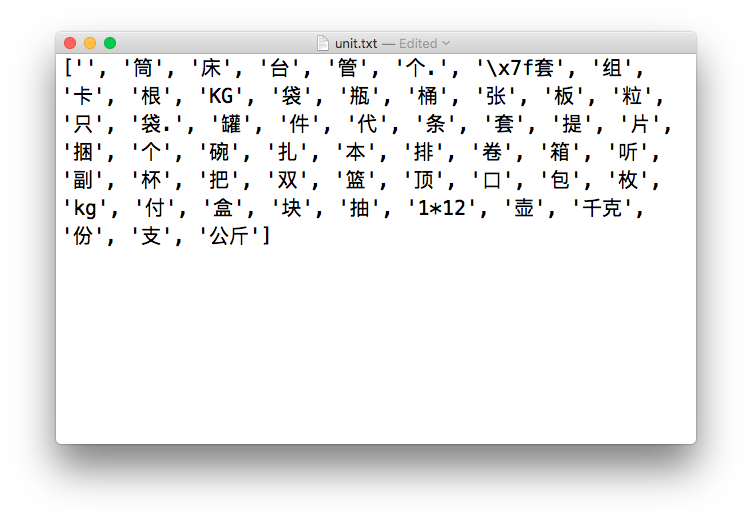
\includegraphics[width=0.9\textwidth]{Nov-16/fig5.png}
    \end{figure}
  \end{frame}
  \begin{frame}{商品名的细分}
    \begin{figure}
      \centering
      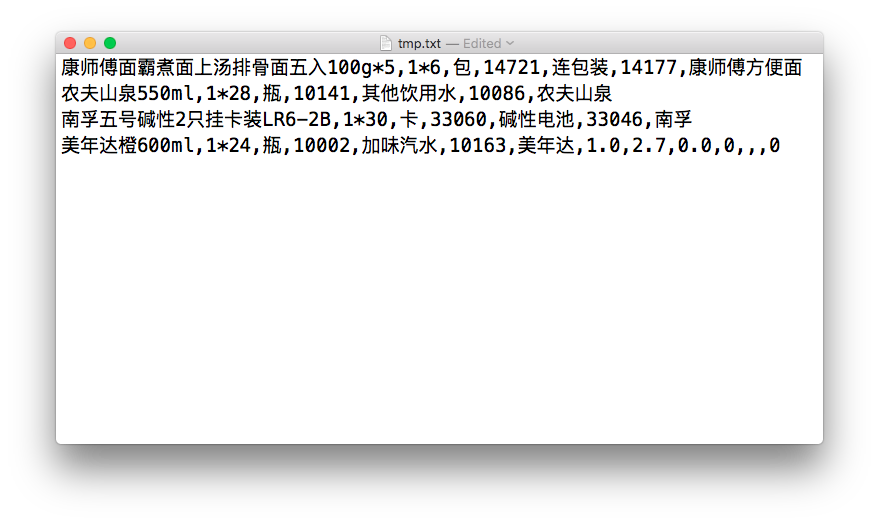
\includegraphics[width=0.9\textwidth]{Nov-16/fig6.png}
    \end{figure}
  \end{frame}
\end{document}

%  \begin{frame}{分词算法的分类}
%    \begin{columns}
%      \begin{column}{0.5\textwidth}
%          基于词典
%      \end{column}
%      \begin{column}{0.5\textwidth}
%        基于统计
%      \end{column}
%    \end{columns}
%  \end{frame}
